% Use only LaTeX2e, calling the article.cls class and 12-point type.

\documentclass[12pt]{article}

% Users of the {thebibliography} environment or BibTeX should use the
% scicite.sty package, downloadable from *Science* at
% www.sciencemag.org/about/authors/prep/TeX_help/ .
% This package should properly format in-text
% reference calls and reference-list numbers.

\usepackage{scicite}

% Use times if you have the font installed; otherwise, comment out the
% following line.

\usepackage{times}
\usepackage{latexsym}
\usepackage{graphicx}
\usepackage{mathptmx}
\usepackage{caption}
\usepackage{subcaption}
\usepackage{pgfplots}
\usetikzlibrary{patterns}
\usepackage{tikz}
\usepackage{multirow}

\usepackage{amsmath}
\usepackage{amsfonts}
\usepackage{amssymb}
\usepackage{amsbsy}
\usepackage{amsthm}
\usepackage{algorithm}
\usepackage{gensymb}
\usepackage[noend]{algpseudocode}
\renewcommand{\algorithmicforall}{\textbf{for each}}

% The preamble here sets up a lot of new/revised commands and
% environments.  It's annoying, but please do *not* try to strip these
% out into a separate .sty file (which could lead to the loss of some
% information when we convert the file to other formats).  Instead, keep
% them in the preamble of your main LaTeX source file.


% The following parameters seem to provide a reasonable page setup.

\topmargin 0.0cm
\oddsidemargin 0.2cm
\textwidth 16cm 
\textheight 21cm
\footskip 1.0cm


%The next command sets up an environment for the abstract to your paper.

\newenvironment{sciabstract}{%
\begin{quote} \bf}
{\end{quote}}


% If your reference list includes text notes as well as references,
% include the following line; otherwise, comment it out.

\renewcommand\refname{References and Notes}

% The following lines set up an environment for the last note in the
% reference list, which commonly includes acknowledgments of funding,
% help, etc.  It's intended for users of BibTeX or the {thebibliography}
% environment.  Users who are hand-coding their references at the end
% using a list environment such as {enumerate} can simply add another
% item at the end, and it will be numbered automatically.

\newcounter{lastnote}
\newenvironment{scilastnote}{%
\setcounter{lastnote}{\value{enumiv}}%
\addtocounter{lastnote}{+1}%
\begin{list}%
{\arabic{lastnote}.}
{\setlength{\leftmargin}{.22in}}
{\setlength{\labelsep}{.5em}}}
{\end{list}}


% Include your paper's title here

\title{SYMBIOTIC TRAFFIC SIMULATION FRAMEWORK} 


% Place the author information here.  Please hand-code the contact
% information and notecalls; do *not* use \footnote commands.  Let the
% author contact information appear immediately below the author names
% as shown.  We would also prefer that you don't change the type-size
% settings shown here.

\author
{Abhinav Sunderrajan,$^{1\ast}$ Vaisagh Viswanathan,$^{1}$ Wentong Cai$^{2}$, Alois Knoll$^{3}$\\
\\
\normalsize{$^{1}$TUM CREATE Ltd}\\
\normalsize{1 CREATE Way 138602, SINGAPORE}\\
\normalsize{$^{2}$School of Computer Engineering}\\
\normalsize{Nanyang Technological University Nanyang Avenue 639798, SINGAPORE}\\
\normalsize{$^{3}$Robotics and Embedded Systems Group Department of Informatics}\\
\normalsize{Technische Universit\"at M\"unchen Boltzmannstra{\ss}e 3 D-85748 Garching bei M\"unchen, GERMANY}\\
\normalsize{$^\ast$To whom correspondence should be addressed; E-mail:  abhinav.sunderrajan@tum-create.edu.sg}
}

% Include the date command, but leave its argument blank.

\date{}



%%%%%%%%%%%%%%%%% END OF PREAMBLE %%%%%%%%%%%%%%%%



\begin{document} 

% Double-space the manuscript.

\baselineskip24pt

% Make the title.

\maketitle 



% Place your abstract within the special {sciabstract} environment.

\begin{sciabstract}
Real time data from several traffic participants such as smart-phone users and vehicles equipped with GPS devices (taxi and bus fleets) is potentially available in the form of a continuous data stream in several mega cities. This real time data can be augmented with that from the traditional sensors for the implementation of several advanced traffic management and control strategies. In this report we present and evaluate a data driven adaptive solution for traffic flow optimization of a real world expressway by employing short-term predictive simulations.
\end{sciabstract}



\section{INTRODUCTION}
A  {\it dynamic data driven adaptive simulation} (DDDAS) incorporates real-time data from the physical system to initialize or steer the simulation system. {\it Symbiotic Simulation}, introduced in~\cite{fujimotoeditors} is a special class of DDDAS involving a mutually beneficial relationship between the physical system and simulation systems. The physical system  provides continuous inputs to steer the simulation which, in turn gives recommendations to the former.

In this report, we present a symbiotic traffic simulation framework which consists of a physical system and prediction \& traffic-flow optimization system. The prediction \& optimization module receives continuous inputs from the physical system, i.e., the road network to initialize predictive faster-than-real-time simulations. Based on the results of the predictive simulations, a recommendation is sent back to control the road network for optimizing traffic flow. The physical system is emulated using a high-fidelity agent based microscopic traffic simulation incorporating acceleration and lane change models. The {\it prediction \& control system} which receives traffic state inputs from the physical system uses a macroscopic traffic flow model to employ a simulation based optimization strategy. The recommendations of this predictive \& control system are given back to the physical system (microscopic simulation) and evaluated for efficacy. Towards this end, the contributions of this report are as follows

\begin{itemize}
\item Develop a framework for symbiotic traffic simulation with the physical system providing continuous inputs to the predictive \& control system while getting back recommendations to optimize traffic flow.
\item Employ the predictive simulations for evaluating several control actions before sending the best recommendation to the physical system. The control action chosen for this proof-of-concept report is {\it ramp-metering}.
\item Evaluate the efficacy of the recommendations given by the predictive \& control system (in the physical system) on employing ramp-metering by simulating a real world expressway.
\end{itemize}

\section{RELATED WORK}
The challenges of incorporating real-time data streams to steer executing simulations have been discussed in~\cite{darema2004dynamic}. Dynamic data driven simulations have found applications in several domains. An emergency detection and response system by~\cite{schoenharl2006wiper} has been developed by processing call data records in real-time for identifying anomalies and emergencies. Plans for further actions when emergencies are detected are determined by agent based simulations. \cite{celik2013dddams} have employed multi-agent data driven simulations for reliable and efficient dispatching of electricity under distributed generation for smart grids. Simulation based short-term forecasting using real-time data streams has found applications in modeling and tracking wildfires by~\cite{douglas2006dddas} and ocean state observation and forecasting by~\cite{patrikalakis2004towards}. 
 
The motivation for a city-scale symbiotic traffic-simulation can be found in \cite{aydt2012symbiotic}. The paper discusses a scenario where hundreds of white-box and gray-box agents provide real-time measurements regarding their geo-location and speed (both white and gray-box agents) and origin-destination (white-box agents only). Considering the burgeoning potential for the availability of traffic data from floating cars and other fixed sensors, it is likely that this real-time data will be beneficial for various ITS based services such as {\it dynamic ramp-metering} which is discussed in this report.

\section{SYSTEM OVERVIEW}
\label{sec:sts}
\begin{figure}[!htbp]
    \centering
    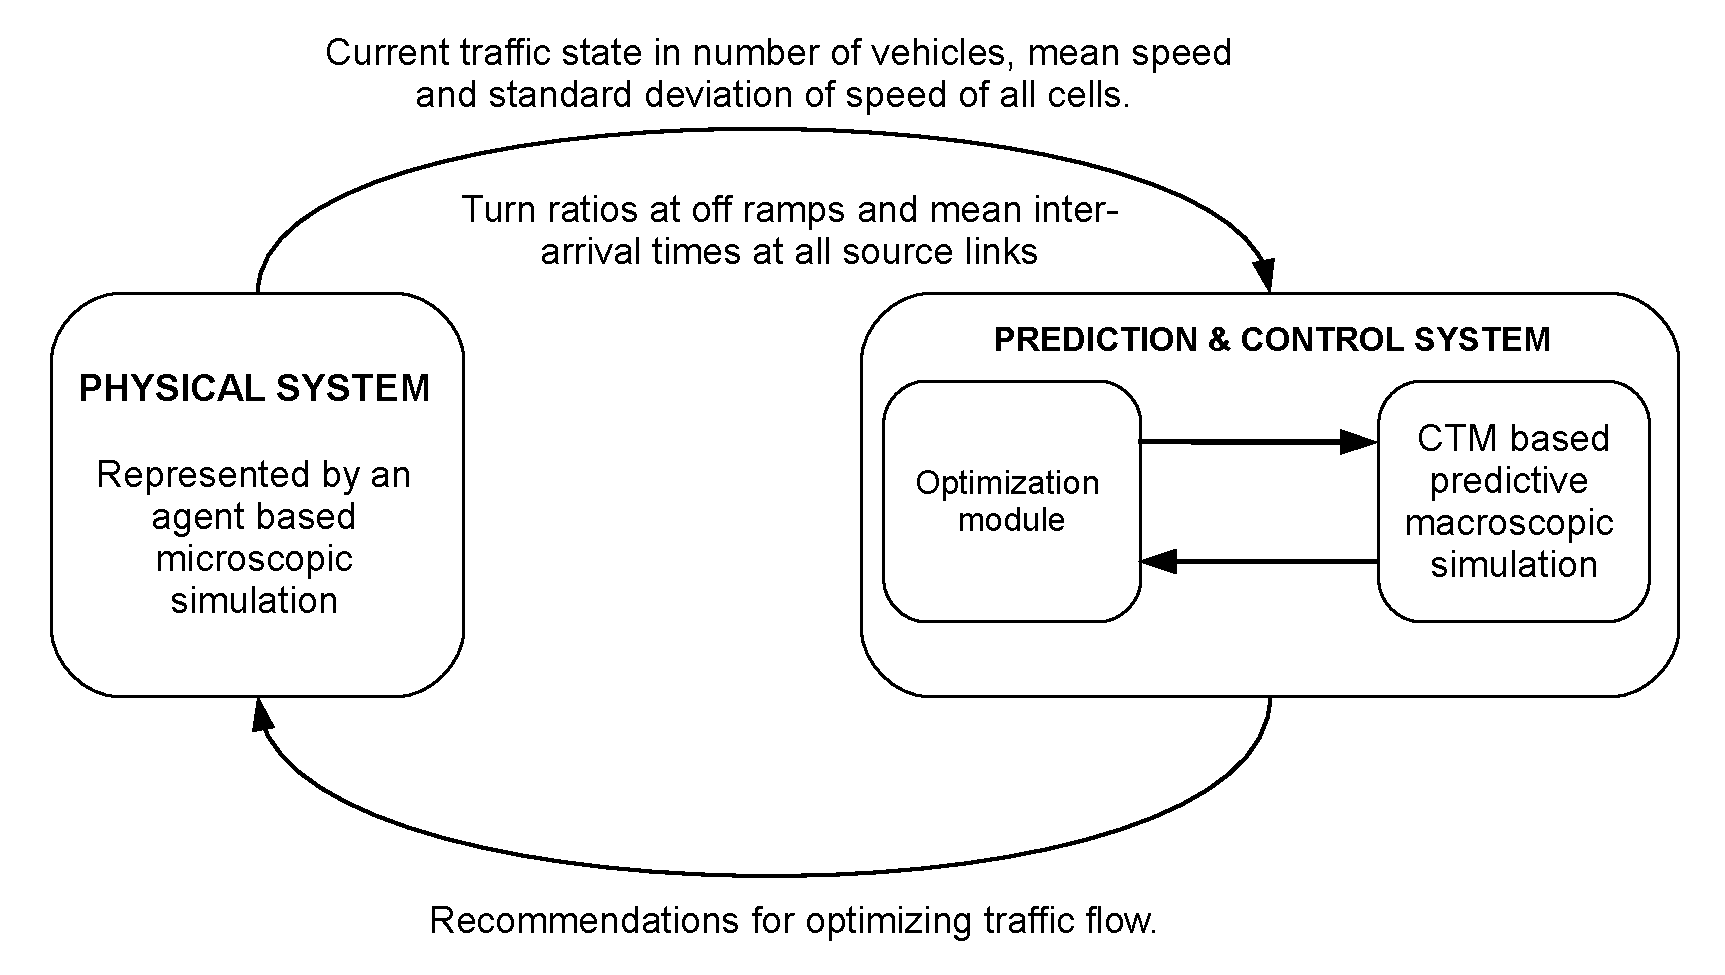
\includegraphics[scale=0.42]{images/methodology.pdf}

    \caption{Symbiotic traffic simulation system.}
    \label{fig:sts-platform}
  \end{figure}

We employ an agent-based microscopic traffic simulation for a realistic representation of the physical world. Microscopic simulations were employed owing to the enormous amount of resources required to implement the recommendations of the predictive simulation on a real world road network. The {\it floating car data} (FCD) provided by the microscopic simulation was used to initialize the state of the predictive {\it Cell Transmission Model} (CTM)~\cite{daganzo1994cell} based macroscopic simulation.  Figure~\ref{fig:sts-platform} illustrates the symbiotic relationship between the physical and the prediction \& control system. 

The predictive component works hand-in-hand with the optimization module to give  recommendations to the physical system to optimize traffic flow after evaluating several candidate solutions. In this report, we optimize the traffic flow of a real world expressway (described in Section~\ref{subsec:pie}) by employing ramp-metering as the control action. The near optimal ramp-metering strategy is determined by the optimization module.

The primary reason for employing a macroscopic simulation for the predictive component, is computational efficiency. A gradient-based optimization strategy involves assessing the fitness of several candidate solutions in parallel. The fitness of a solution is given at the end of a stochastic predictive traffic simulation over a predetermined time horizon.  The above argument motivates us to go in for a cell based macroscopic model despite the relative lack of accuracy in comparison to the microscopic models. The execution time of a CTM based algorithm is proportional to the number of cells simulated thus making it an ideal model for a prediction and control system.

A microscopic traffic model involves simulating hundreds of thousands of agents and updating their speeds and positions at every time-step. Further, modeling lane changes involves acquiring locks (in the context of parallel programming) on multiple lanes making a large scale microscopic simulation computationally expensive (See~\cite{aydt2013multi}). In the subsequent sections we show that our calibrated first-order traffic simulation can model the evolution of traffic state with minimal error (in comparison to the high fidelity microscopic models) provided it is well calibrated and initialized with a reasonably good estimate of the current traffic state in the physical system.

\section{PHYSICAL SYSTEM}
The agent based traffic simulation representing the physical system is based on the {\it SEMSim} platform~\cite{zehe2015semsim,aydt2013multi}. SEMSim is a high fidelity agent-based microscopic simulation. It uses the {\it Intelligent Driver Model} (IDM)~\cite{treiber2010open} and {\it MOBIL}~\cite{kesting2015general} as the acceleration and lane change models respectively. IDM is an accident free model which ensures that a vehicle attains the desired velocity at free flow and maintains the safe bumper to bumper distance to the leading vehicle. It also ensures that the acceleration is an increasing function of the speed and distance to the leading vehicle and a decreasing function of its speed. MOBIL, the lane change model ensures that the resultant accelerations and decelerations for a vehicle and its followers in the old and new lanes does not exceed a safe threshold. A lane change is done only if a vehicle gains speed without violating the safety and inconvenience (to the old and new followers) criteria.


The simulation takes as input a road network detailing the lanes constituting the roads to be simulated. Road segments that don't have a preceding road segment are considered {\it sources} and those without a subsequent segment are {\it sinks}. The traffic thus flows from the sources to the sinks. The route taken by each agent is determined  based on turn ratios (ranging between $0.0$ and $1.0$) specified at each off-ramp. Parameters such as average vehicle length, the acceleration and deceleration terms of IDM are modeled as distributions to take into account heterogeneous driving behaviors and vehicle classes. Note that SEMSim and the term physical system shall be used interchangeably over the rest of this report.

\subsection{SEMSim Parameters}
\label{sec:simparam}

\begin{table}[!htbp]
\centering

\begin{tabular}{ccc}\hline
\textbf{\begin{tabular}[c]{@{}c@{}}Simulation\\ parameter\end{tabular}} & \textbf{Description}                                                                               & \textbf{Value}                                                                                \\ \hline \\
ST                                                                      & Simulation time                                                                                    & 7200 sec                                                                                      \\
$s_{0}$                                                                 & \begin{tabular}[c]{@{}c@{}}Minimum bumper-to-bumper distance \\ to the front vehicle.\end{tabular} & $2.0$ m                                                                                       \\
T                                                                       & Time gap to preceding agent                                                                        & $1.4$ sec                                                                                     \\
$l_{i}$                                                                       & Vehicle length                                                                  & \begin{tabular}[c]{@{}c@{}}Normal distribution with \\ $\mu=3.0$ m and $\sigma=0.1$ m\end{tabular} \\
$V_{0}$                                                                 & Desired speed of agent                                                                            & $20$ m/s                                                                                      \\
a                                                                       & Maximum acceleration term for IDM                                                                  & \begin{tabular}[c]{@{}c@{}}Uniform distribution between \\ $1.2$ and $1.6~m/s^2$\end{tabular} \\
b                                                                       & Maximum deceleration term for IDM                                                                 & \begin{tabular}[c]{@{}c@{}}Uniform distribution between \\ $1.8$ and $2.2~m/s^2$\end{tabular} \\
$p_{0}$                                                                 & Politeness factor for MOBIL                                                                       & 0.3                                                                                           \\
$\Delta a_{th}$                                                         & Lane change threshold for MOBIL                                                                   & $0.3 ~m/s^2$                                                                        \\ \hline          
\end{tabular}
\caption{The microscopic simulation parameters}
\label{table:sim-param}
\end{table}


SEMSim  was initialized with the parameters listed in Table~\ref{table:sim-param}. Parameters such as $a$, $b$ and $l_{i}$ are modeled as distributions to take into account heterogeneous driving behaviors and vehicle classes.




\section{MODELING OF PREDICTION SYSTEM}
The predictive, faster-than-real-time macroscopic simulation is based on the stochastic variant of the Cell Transmission Model~\cite{boel2006compositional} and METANET~\cite{kotsialos2002traffic}. The cell network, $\mathbb{C}$ is comprised of $n$ cells. At each time instant, $t=k.T_{ctm}$, $k=0,1, .... K$ (where $K$ is the time horizon) the state of all cells are updated. The discrete event time step is denoted by $T_{ctm}$.
  
The state of a cell $c_i\in \mathbb{C}$ at each time step $k$ is determined by {\it sending} $S_i(k)$ and {\it receiving potentials} $R_i(k)$. $S_i(k)$ and $R_i(k)$ represent the number of vehicles cell $c_i$ can send and receive at time-step $k$. The mean and standard deviation of speed for a cell $c_i$ are denoted by $v_i(k)$ and $v_i^{\sigma}(k)$ respectively.  The number of vehicles in a cell $c_i$ at time-step $k$ is given by $N_{i}(k)$. While $N_i^{max}(k)$ represents the maximum number of vehicles that can be accommodated in cell $c_i$ given an average speed of $v_i(k)$. $N_i^{max}(k)$ is given by
\begin{equation}
\label{eq:nmax}
N_i^{max}(k)=\frac{l_i.\lambda_i}{T_{gap}.v_{i}(k)+ L_{eff}}
\end{equation}
where $L_{eff}$, the {\it effective} vehicle length represents the sum of mean vehicle length and minimum gap. $T_{gap}$ represents the safe time gap.
The length of cell $c_i$ is denoted by $l_i$ which is a variable and subject to the constraint $l_i \le V_0^i\times T_{ctm}$. $V_0^i$ is the constant free-flow speed for the cell. This constraint ensures that no vehicle can enter and exit a cell within one time-step. The number of lanes in cell $c_i$ corresponding to the associated road-link is denoted by $\lambda_i$. The outflow in number of vehicles at time-step $k$ from cell $c_i$ is given by $y_i(k)$ and the density in number of vehicles per unit distance per lane is denoted by $\rho_i(k)$. The {\it critical density} $\rho^{crit}_i$ separating free and congested traffic of a cell $c_i$ is given by 
\begin{equation}
\label{eq:critden}
\rho^{crit}_i=\frac{1}{V_0^i.T_{gap}+L_{eff}}
\end{equation}

\begin{algorithm}[!htbp]
\caption{CTM based macroscopic predictive simulation.}
\label{algo:ctm}

\begin{algorithmic}[1]

\While{$t<K$}
\ForAll{$c_i \in \mathbb{C}$}
\State update sending and receiving potentials.
\EndFor

\ForAll{$c_i \in \mathbb{C}$}
\State update outflow.
\EndFor

\ForAll{$c_i \in \mathbb{C}$}
\State update number of vehicles.
\State update density.
\EndFor

\ForAll{$c_i \in \mathbb{C}$}
\State update average speed $v_{i}$
\State update the maximum number of vehicles $N^{max}_{i}$
\EndFor

\State $t=t+k.T_{ctm}$
\EndWhile


\end{algorithmic}
\end{algorithm}
Other constants in this predictive simulation are the terms $\kappa, \delta$ and $\phi$. The constants $\kappa$ and $\delta$ adapt the speed of the vehicles after an on-ramp expressway merge while last term $\phi$ adapts the speed of cell where a lane drop occurs. $V^{out}_{min}$ denotes the minimum speed of cell a when it is completely congested. $V^{out}_{min}$ thus models the fact that some vehicles exit a bottleneck with a minimum speed. Finally, $A_{m}$ is a parameter of the fundamental diagram representing the speed density relationship (See~\cite{kotsialos2002traffic}).


\begin{figure}[!htbp]
    \centering
    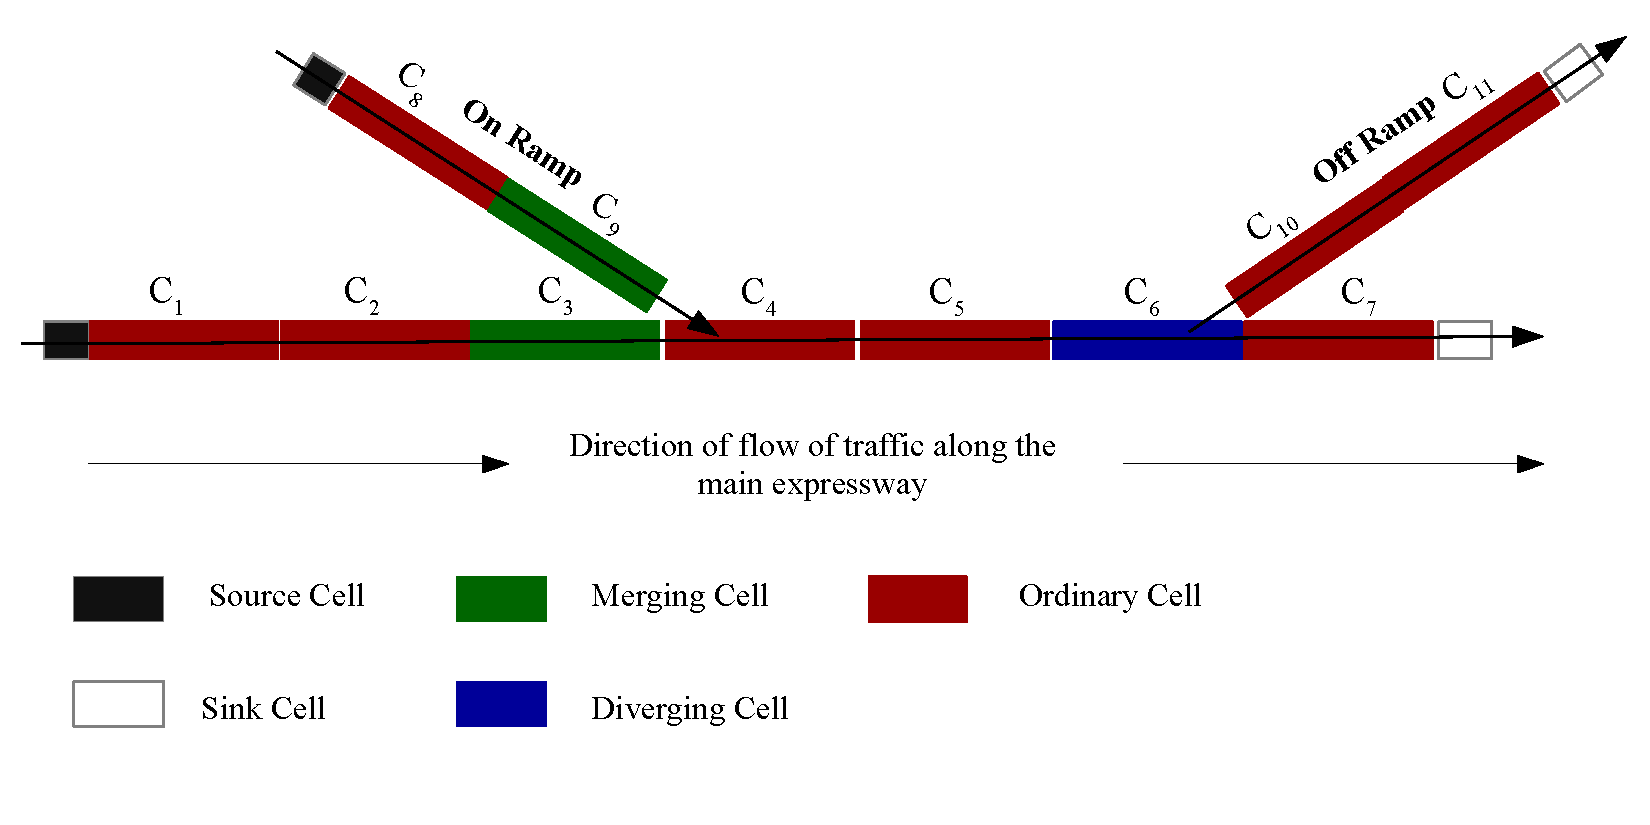
\includegraphics[scale=0.5]{images/cellNetwork.pdf}

    \caption{An illustrative cell network.}
    \label{fig:cell-network}
\end{figure}
  
The cells constituting the cell network $\mathbb{C}$ are classified into five different types as shown in Figure~\ref{fig:cell-network}. Note that this is an illustrative network and not the real world expressway (see Section~\ref{subsec:pie}) simulated for the experiments. The {\it Merging} cells are associated with the parameter {\it merge priority} $\mu\in [0.0,1.0]$ which controls the proportion of vehicles that moves to the next cell in a given time-step. Correspondingly $\mu^{on}_{ramp}$ and $\mu_{exp}$ are the merge priorities of the on-ramp and expressway cells respectively. The {\it source} and {\it sink} cells are not physically related to any of the road links. The source and sink cells are effectively {\it ghost cells} since they have zero length and zero lanes. The former injects agents into the simulation while the agents exit the simulation through the latter. A {\it Diverging} cell is associated with the turn ratios $\tau$ ranging between $0.0$ and $1.0$ representing the proportion of vehicles exiting the expressway through off ramp and those continuing to traverse along the expressway. Cells $C_3$ and $C_9$ are considered {\it predecessors} of cell $C_4$. Similarly, cells $C_{10}$ and $C_7$ are considered {\it successors} of cell $C_6$.

Algorithm~\ref{algo:ctm} shows the progress of the simulation over the prediction time horizon $K$. The equations governing the state of all cells at each time step are provided in the Appendix~\ref{appendix:a}.



\section{OPTIMIZATION MODULE}
\label{sec:optimization}

\begin{algorithm}[!htbp]
\caption{Particle Swarm Optimization}
\label{algo:ramp-metering}

\begin{algorithmic}[1]
\State $swarmSize$, $maxiter\leftarrow$ swarm size and maximum iterations for PSO respectively.
\State $\mathbb{P}\leftarrow \varnothing$, the set of particles in the swarm.
\State $\alpha \leftarrow$ proportion of velocity to be retained.
\State $\beta \leftarrow$ proportion of personal best to be retained.
\State $\gamma \leftarrow$ proportion of informant's to be retained.
\State $\delta \leftarrow$ proportion of global best to be retained.


\For{$swarmSize$ times}
	\State $\mathbb{P} \leftarrow~\mathbb{P}\bigcup$ {new particle $\vec{x}$ with initial velocity $\vec{v}$}
\EndFor	

\State $\vec{Best}\leftarrow\varnothing$
\State $iter\leftarrow0$

\Repeat

\ForAll{$\vec{x}\in\mathbb{P}$}
\If{$\vec{Best}==\varnothing$ {\it or} $fitness(\vec{x})<fitness(\vec{Best})$}
\State $\vec{Best}\leftarrow \vec{x}$
\EndIf
\EndFor

\State$\mathbb{Z}\leftarrow~\varnothing$

\ForAll{$\vec{x}\in\mathbb{P}$ with velocity $\vec{v}$}
\State $\vec{x}^{\,*}$ previous fittest location of $\vec{x}$
\State $\vec{x}^{\,+}$ previous fittest location of informants of $\vec{x}$
\State $\vec{x}^{\,!}$ previous fittest location of any particle

\ForAll{$x_i\in\vec{x}$}
\State $b\leftarrow$ random number $0.0$ to $\beta$ inclusive
\State $c\leftarrow$ random number $0.0$ to $\gamma$ inclusive
\State $d\leftarrow$ random number $0.0$ to $\delta$ inclusive
\State $v_i\leftarrow \alpha v_i+b(x_{i}^{*} - x_i)+c(x_{i}^{+} - x_i)+d(x_{i}^{!} - x_i)$
\EndFor

\EndFor

\ForAll{$\vec{x}\in\mathbb{P}$}
\State $\vec{x}\leftarrow \vec{x}+\vec{v}$
\EndFor
\State $iter\leftarrow iter+1$
\Until{$iter<maxiter$}
\State \Return $\vec{Best}$
\end{algorithmic}
\end{algorithm}

We implemented a {\it particle swarm optimization} (PSO)~\cite{weise2009global} approach (Algorithm~\ref{algo:ramp-metering}) for the optimization module to determine the best control strategy for the case study described later in Section~\ref{sec:case-study}.
The PSO algorithm seeks to identify the best control-action by minimizing the value returned by the function $fitness(\vec{x})$ ($\vec{x}$ represents a candidate solution) running the CTM based predictive simulation over a time horizon $K$. Specifically, the fitness function returns the value $J$ (Equation~\ref{eq:minimize}) which represents the weighted average of {\it total time spent} (TTS) and {\it total distance traveled} (TTD) over the time horizon $K$ and over $M$ cells~\cite{hadiuzzaman2013cell}.



 

\begin{equation}
\label{eq:minimize}
J=T.\sum\limits_{\substack{k=0}}^{K}\sum\limits_{\substack{i=1}}^{M}\lambda_i.l_i[\alpha_{TTS}\rho_i(k)-\alpha_{TTD}.\rho_i(k).v_i(k)]
\end{equation}

The algorithm seeks to minimize the total number of vehicles while maximizing traffic flow over $K$. Note that $\alpha_{TTS}$ \& $\alpha_{TTD} \in (0.0,1.0)$. The PSO algorithm is a population-based method where existing population members (or particles) are tweaked in response to new discoveries in the search space. At each iteration, the fitness of every individual (Equation~\ref{eq:minimize}) is assessed using the predictive simulation. Each particle is then tweaked based on the best global, {\it informant's} and personal solutions obtained thus far. The informants of a particle $\vec{x}$ refer to a small subset of particles from the population which are chosen randomly each at iteration.


\section{CASE STUDY}
\label{sec:case-study}
\subsection{Ramp Metering}
\label{subsec:ramp-metering}
Ramp-metering is a traffic control mechanism implemented in several cities across the world to reduce the congestion on expressways~\cite{bogenberger1999advanced}. Ramp meters are traffic signals placed at the intersection of on-ramps and expressways. They regulate the flow of vehicles along the ramps so as to minimize the turbulence caused due to merging vehicles disrupting the mainline flow. Care must be taken to ensure that the queue of the vehicles waiting along the on-ramps does not spill into the preceding urban street network. 

Ramp-metering strategies are classified into two types: {\it fixed-time} and {\it reactive}~\cite{papageorgiou2003review}. The fixed time strategy is based on historical data pertaining to flow rates along the on-ramps and the expressway at different times of the day. The main drawback of the fixed time strategy is that their settings are based on historic rather than real time data. It does not take into account the varying nature of traffic demand and the occurrence of events such as accidents and road blocks which could cause massive congestions. 

Reactive ramp-metering strategies aim to optimize the flow of traffic based on real-time measurements. Reactive ramp-metering is classified into two types: {\it Local Ramp-Metering} and {\it Multivariable Regulator Strategies}~\cite{papageorgiou2003review}. The former makes use of measurements in the vicinity of an on-ramp to regulate the flow on the ramp. The control strategy applied for an on-ramp is independent of the measurements and controls applied in other on-ramps in the vicinity. The latter makes use of the system wide measurements to simultaneously regulate traffic flow along all on-ramps. A review on several implemented and proposed ramp-metering strategies can be found in~\cite{bogenberger1999advanced}.

In this report we employ particle swarm optimization described in Section~\ref{sec:optimization} to develop a system wide ramp-metering strategy of a real world expressway by regulating the flow on all on-ramps simultaneously. The system-wide ramp controller designed for this report determines the maximum allowable {\it queue-threshold} $q^{th}_r$ (Equation~\ref{eq:constraint}) for a ramp $r\in \mathbb{R}^{on}_{ramps}$ before turning the phase of the signal to green from red, where $\mathbb{R}^{on}_{ramps}$ is the set of controllable on-ramps in the system.

\begin{equation}
 \label{eq:constraint}
\frac{N_r(k)}{N^{max}_r(k)}\le q^{th}_r
 \end{equation}

 Where $N_r(k)$ and $N^{max}_r(k)$ is the number and the maximum number of vehicles on the on-ramp $r$ at time step $k$. $N^{max}_r(k)$ at time-step $k$ is determined from Equation~\ref{eq:nmax}. Concretely, the task is to find the ideal value of $q^{th}_r$ for all on-ramps so as to minimize $N_{total}$. Note that $q^{th}_r \in [0.0,1.0]$.


\subsection{Simulated Physical Environment}
\label{subsec:pie}
\begin{center}
\begin{figure}[!htbp]
    \centering
    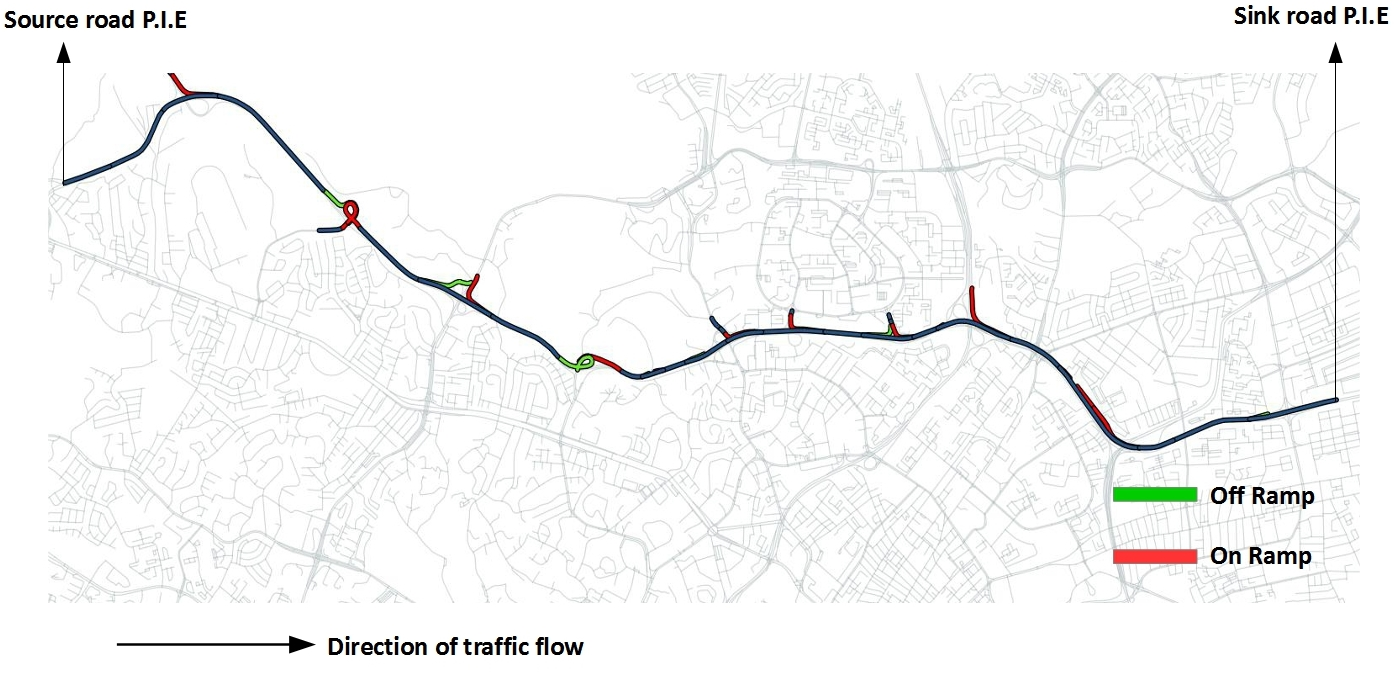
\includegraphics[scale=0.40]{images/PIE.jpg}

    \caption{Simulated section of P.I.E (Singapore) and location of all on/off ramps.}
    \label{fig:pie-changi}
  \end{figure}
\end{center}
For the experiments in this report, we simulate a $13$ km stretch of P.I.E (Pan Island Expressway) in central Singapore (Figure~\ref{fig:pie-changi}) with all on and off ramps. The on ramps and the first P.I.E link are sources, while all off ramps and the last link on P.I.E are sinks. Refer to the Table~\ref{fig:pie-changi} for the location of all on/off ramps (or {\it static bottlenecks}) starting from the beginning of the first road-segment on P.I.E. The average distance between two bottlenecks is around $565\text{~m}$ along this stretch of P.I.E. The turn ratios for all off-ramps is kept constant at $0.25$. This implies that $25\%$ of all vehicles exit at a given off ramp while the remaining $75\%$ of the vehicles continue to travel on the main expressway. The number of lanes in the simulated stretch of the expressway varies between $3$ and $6$.



\begin{table}[!ht]
 \centering
\begin{tabular}[b]{ccc}\hline
      {\bf DISTANCE} (m) & {\bf RAMP TYPE} \\ \hline
     583.98 & On Ramp \\ 
     1973.35 & Off Ramp \\ 
     2489.87 & On Ramp \\ 
     3261.27 & Off Ramp \\ 
     4071.9 & On Ramp \\ 
     4834.84 & Off Ramp \\ 
     5531.18 & On Ramp \\ 
     5743.11 & Off Ramp \\ 
     5965.29 & On Ramp \\ 
     6207.74 & Off Ramp \\ \hline
     \end{tabular}
     \quad
     \begin{tabular}[b]{ccc}\hline
       {\bf DISTANCE} (m) & {\bf RAMP TYPE} \\ \hline
     7025.15 & On Ramp \\ 
     7658.4 & On Ramp \\ 
     8040.83 & Off Ramp \\ 
     8554.28 & On Ramp \\ 
     8807.94 & Off Ramp\\ 
     9591.84 & On Ramp \\ 
     10148.24 & Off Ramp \\ 
     11286.2 & On Ramp \\ 
     11637.04 & On Ramp \\ 
     12438.23 & Off Ramp \\  \hline
    \end{tabular}
      \caption{Location of all On/Off ramps along the expressway.}
      \label{table:on-off-ramp}
\end{table}



\subsection{Traffic Scenario}
\label{subsec:traffic-scenario}
 \begin{table}[!htbp]
 \caption{Mean inter-arrival times at all source links/cells}
 \begin{tabular}[b]{ccc}\hline
       {\bf DISTANCE} (m) & {\bf RAMP TYPE} & {\bf $\epsilon_s$} (sec)\\ \hline
      0.0 & First P.I.E link & 1.0\\
      583.98 & On-Ramp & 2.0\\ 
      2489.87 & On-Ramp & 3.6\\ 
      4071.9 & On-Ramp & 3.6\\ 
      5531.18 & On-Ramp & 3.6\\ 
      5965.29 & On-Ramp & 3.6\\ \hline
      \end{tabular}
      \quad
      \begin{tabular}[b]{ccc}\hline
        {\bf DISTANCE} (m) & {\bf RAMP TYPE}& {\bf $\epsilon_s$} (sec) \\ \hline
      7025.15 & On-Ramp & 2.0\\ 
      7658.4 & On-Ramp & 2.0\\ 
      8554.28 & On-Ramp & 3.6\\ 
      9591.84 & On-Ramp & 3.6\\ 
      11286.2 & On-Ramp & 3.6\\ 
      11637.04 & On-Ramp & 3.6\\ \hline
     \end{tabular}
       \label{table:iat}
 \end{table}
 
  The traffic state of the expressway at the end of a time horizon is determined by the inter-arrival time $\epsilon_s$ for all source links and cells. The stretch of the expressway simulated consisting of $11$ on-ramps and along with the first expressway link has $12$ source links/cells. Table~\ref{table:iat} lists the mean inter-arrival times for all source links/cells. Notice that the flow of vehicles into the expressway along all on-ramps  are significantly less (1000 vehicles/hour) except for the ones at $583$ m, $7025$ m and $7658$ m. The optimization module thus needs to find a ramp metering strategy which balances the flow along all on-ramps so as to minimize the surge of vehicles along the three ramps with relatively higher inflow of vehicles.


\section{RESULTS}
\label{sec:experiments}

\subsection{Calibration of Predictive Simulation}

To ensure that the state predicted by the macroscopic simulation accurately represents the state of the physical system, the model parameters have to be calibrated. We need to identify (and tune) the parameters which will have significant impact in terms of bridging the difference in the state of the physical system and that of the predictive simulation at the end of a given time horizon.

Towards this end we simulated SEMSim representing the physical system over a time horizon $K=2000$ seconds. The mean inter-arrival times of all source links $\epsilon_s$ were kept constant during the time period of the simulation. There are no vehicles in the simulation at time-step $k=0$. $N_i^{semsim}(K)$ denotes the number of vehicles in each cell of the mainline expressway (corresponding to the cell-network associated with the predictive system) is computed at the end of the microscopic agent-based simulation. 

The initial state and the mean inter-arrival times of vehicles for all source cells $\epsilon_{s}$ are the same as SEMSim for the predictive simulation. The turn ratios at the off-ramp ($\tau_{ramp}^{off}$) and expressway ($\tau_{exp}$) intersections are also the same as that of the physical system. The time-step $T_{ctm}$ for the predictive simulation is kept constant at $4.0$ seconds. To identify and then tune the parameters which bridge the difference between the predictive simulation and the physical system, we attempt to minimize the least square error given by Equation~\ref{eq:calibration}
\begin{equation}
\label{eq:calibration}
\sqrt{\sum\limits_{i=1}^{i=n_{exp}}(N_i^{semsim}(K)-N_i^{ctm}(K))^2}
\end{equation}
Where $N_i^{ctm}(K)$ denotes the number of vehicles in each cell of the mainline expressway computed at the end of the predictive simulation time horizon $K$. The least square error thus represents the difference between the number of vehicles for all expressway cells (numbering $n_{exp}$) at $K$. We ran the predictive simulation $1500$ times to the return least square error for each of these runs to generate $1600$ data points. The parameters of the CTM based predictive simulation were varied based on the range column of the Table~\ref{table:pred-sim-var}.


\begin{table}[!htbp]
\centering
\caption{The predictive simulation parameters}
\label{table:pred-sim-var}
\begin{tabular}{cclc}\hline
\textbf{\begin{tabular}[c]{@{}c@{}}Simulation \\ parameter\end{tabular}} & \textbf{Description}                                                                     & \multicolumn{1}{c}{\textbf{Range}} & \textbf{\begin{tabular}[c]{@{}c@{}}Calibrated\\ Value\end{tabular}} \\
\hline \\
$\mu_{ramp}$                                                             & \begin{tabular}[c]{@{}c@{}}Merge priority for on ramp \\ merging cells\end{tabular}      & $[0,1, 0.7]$                       & 0.45                                                                \\
$\mu_{exp}$                                                              & \begin{tabular}[c]{@{}c@{}}Merge priority for express way \\ merging cells.\end{tabular} & $[0.8, 0.1]$                       & 0.9                                                                \\
$T_{gap}$                                                                & Safe time gap for vehicles (s)                                                           & \multicolumn{1}{c}{$[1.2, 1.5]$}   & $1.25$                                                              \\
$V^{out}_{min}$                                                          & Minimum speed in a cell (m/s)                                                            & $[2.0, 6.0]$                       & 2.5 m/s                                                             \\
$\delta$                                                                 & On ramp merge term                                                                       & $[0.02, 0.6]$                      & 0.27                                                                \\
$A_{m}$                                                                  & Model term of fundamental diagram                                                        & \multicolumn{1}{c}{$[1.0, 4.0]$}   & $2.34$                                                              \\
$\phi$                                                                   & Lane drop term                                                                           & $[1.8, 3.6]$                       & 2.7  \\
$\kappa$                                                                   & On ramp merge term                                                                           & $[0.1, 2.0]$                       & 0.45  \\ \hline                                                              
\end{tabular}
\end{table}

 
\begin{equation}
\label{eq:regression}
LSE=\beta_0-\beta_1.\mu^{on}_{ramp}+\beta_2.T_{gap}+\beta_3.T_{gap}^2+\beta_4.T_{gap}.\mu^{on}_{ramp}
\end{equation}

The polynomial regression  with an $R^2$ Statistic (a measure of model fit indicating the percentage of variance explained by the model) of $0.817$ is shown in Equation~\ref{eq:regression}. This model clearly shows that the two dominant terms are $T_{gap}$ and $\mu^{on}_{ramp}$. Based on the results of the calibration, the CTM based predictive simulation was initialized with the parameters shown in Table~\ref{table:pred-sim-var}.  The values of $A_m, \phi, \kappa$ and $\delta$ are chosen based on the calibration experiments by ~\cite{kotsialos2002traffic}. Note that $V_{min}^{out}$ is set to $0.0$ for the on-ramps since the vehicles come to a complete standstill when the signal is red.




\subsection{Efficacy of Ramp Metering}
\label{subsec:results}

In this section, we quantify the efficacy of using ramp-metering in the physical system (SEMSim) based on the recommendations given by the predictive \& control system. As discussed in Section~\ref{subsec:ramp-metering}, we need to find the optimal value of $q^{th}_r \in [0.0,0.8]$ for each of the $11$ on-ramps for the environment simulated. Note that the maximum value of the queue-threshold $q^{th}_{max}$ is set to $0.8$. The controller sets the phase to green when $q^{th}_r$ exceeds $q^{th}_{max}$ serving as the first constraint. The other constraints are
\begin{enumerate}
\item The minimum phase time for both the red and green phases are $12$ seconds.
\item The signal at an on-ramp can be continuously red only for a maximum of $120$ seconds. After a $120$ second red phase, there is a mandatory green phase for $24$ seconds.
\end{enumerate}
The first of the above constraint ensures that the phase changes do not change rapidly. This gives adequate reaction times for drivers to slow down and accelerate at an intersection. The second constraint ensures that none of the vehicles wait at an on-ramp for an inordinately long time thus preventing the starvation of an on-ramp $r$ even if the $q^{th}_r$ is not exceeded.

The fitness function $fitness(\vec{x})$ from Algorithm~\ref{algo:ramp-metering} has been modified to compute $J^{mean}$, the mean of $5$ different runs of CTM for a ramp-metering configuration $\vec{x}$ to account for model stochasticity. Note that the term {\it run of the predictive simulation} refers to the execution of the simulation over the time horizon $K$. The initial population size was set to $15$ and the maximum number of iterations was restricted to $25$ (based on Figure~\ref{fig:ctm-improvement}). The parameters $\alpha, \beta, \gamma$ and $\delta$ were set to $0.9$, $2.0$, $2.0$ and $2.0$ respectively.  The parameters in $\alpha_{TTS}$ and $\alpha_{TTD}$ used to compute the fitness (Equation~\ref{eq:minimize}) $J$ are set to $0.95$ and $0.05$ respectively.


\begin{figure}[!htbp]
    \centering
    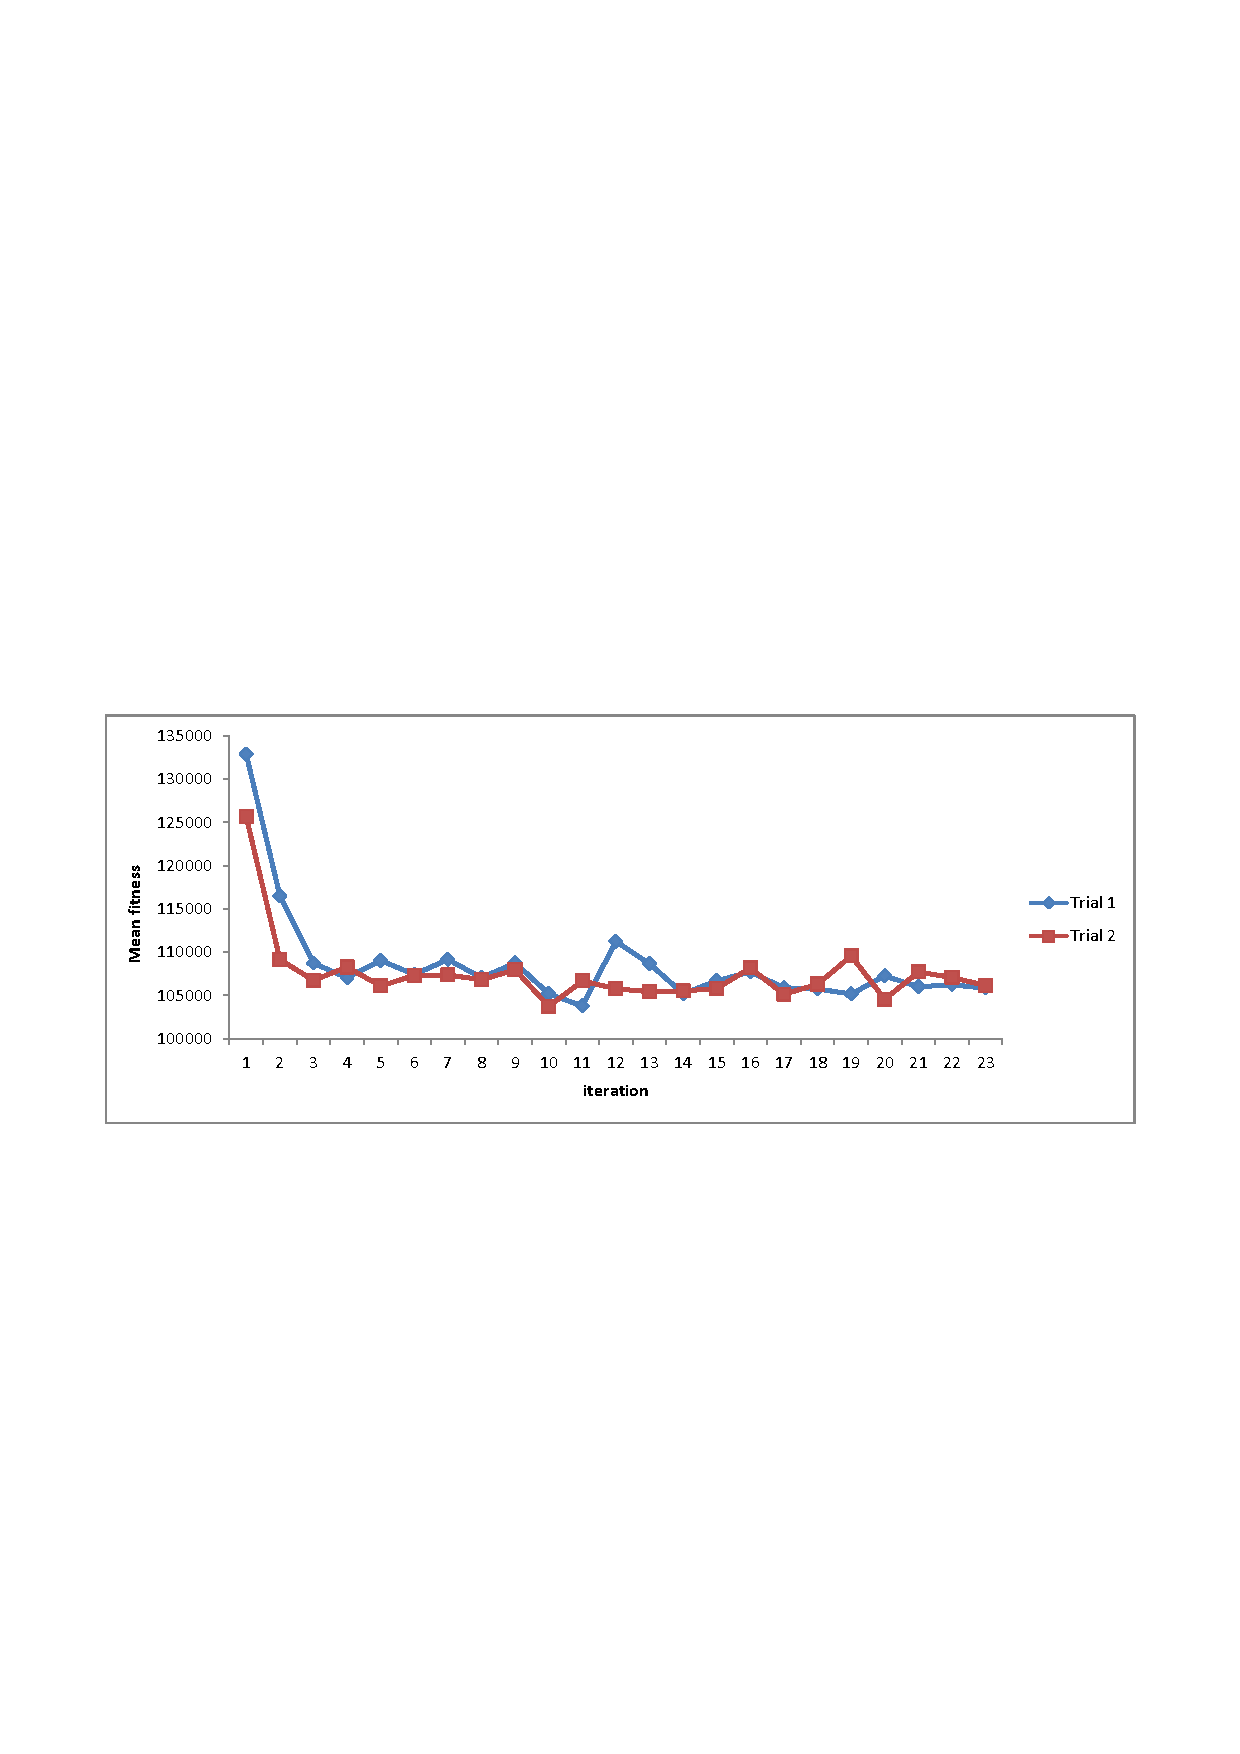
\includegraphics[clip=false,scale=0.75]{images/CTM-improvement-PSO.pdf}
   \caption{$J^{mean}$ vs iteration.}
   \label{fig:ctm-improvement}
 \end{figure}
  
Figure~\ref{fig:ctm-improvement} plots $J^{mean}$ as a function of iteration count for two different trials of the PSO algorithm running the CTM based predictive simulation. It can be observed that the algorithm converges to a large extent in less than $25$ iterations. 
The best ramp-meter configuration (determined using the predictive simulation) is now given as a recommendation to SEMSim which returns the corresponding $J$ over the same time horizon of $1800$ seconds. Note that the constraints pertaining to phase timings are implemented in SEMSim as well. In the next section, we determine the percentage improvement (in terms of $J$) over the no ramp metering case when the recommendation of the predictive system is fed back to the physical system.


  
  \begin{figure}[!htbp]
      \centering
      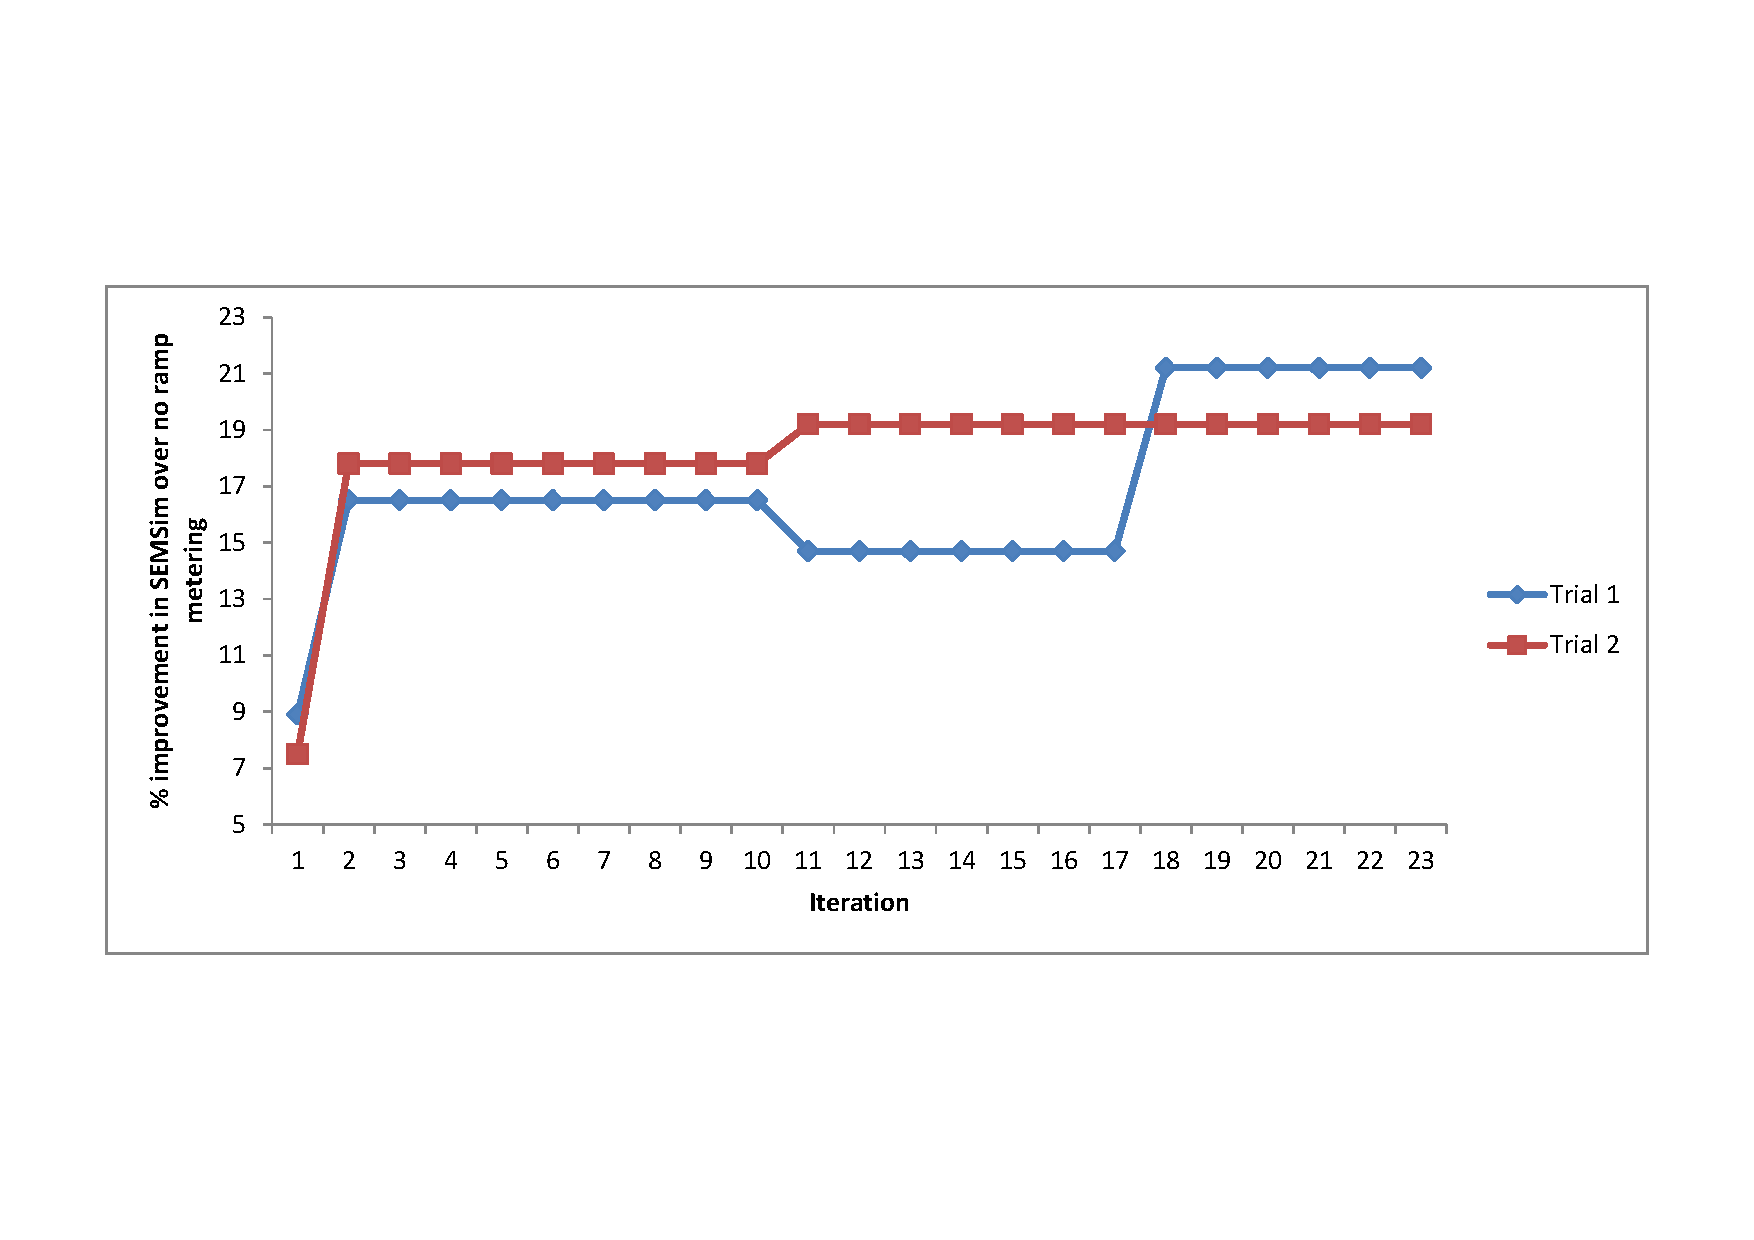
\includegraphics[clip=false,scale=0.52]{images/SEMSim-improvement-PSO.pdf}
              \caption{Percentage improvement in $J$ when recommendations are given to SEMSim.}
      \label{fig:semsim-improvement}
    \end{figure}

 Figure~\ref{fig:semsim-improvement} shows the percentage improvement of $J$ over the no ramp-metering case (corresponding to the two trials in Figure~\ref{fig:ctm-improvement}) when the recommendations of the prediction \& control system (in terms of the global best solution obtained thus far) are fed back into SEMSim. Assuming that the optimization module was invoked at time $T$ and its execution over $iter$ iterations takes $\Delta T$ seconds, the recommendations should be given to SEMSim at $T+\Delta T$ and evaluated until $T+K-\Delta T$ to return $N_{total}$. For our experiments, we ignored $\Delta T$ since it is small ($42$ seconds) and we do not expect the traffic conditions to change drastically over $\Delta T$ given the constant inter-arrival times at all source links/cells.  
 
Improvements in the  range of around $17\%$ and beyond is observed at the end of $10$ iterations in both trials. To validate our approach further, we gave a bad recommendation to the physical system where $q^{th}_r$ was set to $q^{th}_{max}$ for all $r\in \mathbb{R}$. The erroneous recommendation resulted in $J^{mean}$ (for the physical system) increasing by $43\%$ indicating worsening of traffic flow. The results in this section  illustrates the potential of symbiotic traffic simulation as an effective tool for traffic flow optimization through dynamic ramp-metering as a case study.

\subsection{Note On The Computational Efficiency of Predictive Simulation}

A data driven adaptive simulation and prediction framework for traffic systems should work under reasonable time constraints for predicting short term evolution of state and giving back recommendations to optimize traffic flow. The simulations employed by the predictive system should thus be reasonably fast. The computational time for the CTM based simulation (used for determining $J$) over a time horizon of $1800$ seconds is around $75$ milliseconds. The CTM simulation was coded in Java SE 7 and measured in a 2.5 GHz Intel i5 system running on Windows 7. The entire run of the PSO algorithm over $25$ iterations took around $45$ seconds to complete, thus satisfying the soft real time constraints for a symbiotic traffic simulation. The prediction \& control system can give a recommendation much earlier (at the end of $40$ iterations) to the physical system before searching for and further fine tuning the ramp control strategy in the background.


\section{CONCLUSIONS \& FUTURE WORK}
\label{sec:conclusion}
In this work we have established that data driven predictive simulations can be beneficial towards optimizing traffic flow.  The prediction and optimization system should receive fairly accurate and continuous information on the current traffic state. This information is used for initialization, calibration and steering of the predictive simulations. Accurate current state estimation in turn increases the accuracy of the short term predictions (of evolution of traffic flow) thereby increasing the efficacy of the suggested control measures. Data from traditional fixed sensors can be augmented with FCD from smart phones and vehicle fleets such as taxis and public buses for enhanced traffic state reconstruction. The simulation model and optimization strategy used in the prediction \& control system can be varied depending upon accuracy, efficacy and computational time constraints.

Symbiotic traffic simulations also offer exciting opportunities to implement and optimize several techniques for traffic flow optimization (other than ramp-metering discussed in this report) such as adaptive speed limits and dynamic routing. Mobile applications and in car navigation systems provide a great means to disperse information to the traffic participants while the control system receives user anonymized data about vehicle speed, location and even origin-destination flows. This form of a symbiotic simulation based traffic prediction and optimization framework directed towards dispersing and receiving updates from individual drivers will be the focus of our future research.


\section{APPENDIX. EQUATIONS FOR UPDATING CELL STATE}
\label{appendix:a}

\textbf{Updating Sending and Receiving Potentials for all $c_i\in \mathbb{C}$}
\begin{subequations} 
\label{eq:sp-rp}
\begin{eqnarray}
term_1=\frac{N_i(k).v_i(k).T_{ctm}}{l_i}\\
term_2=\frac{N_i(k).V^{out}_{min}.T_{ctm}}{l_i}\\
S_i(k+1)= min(max(term_1,~term_2),~N_i(k))\\
R_i(k+1)=N_i^{max}(k)-N_i(k)
\end{eqnarray}
\end{subequations}


\textbf{Updating the outflow for all $c_i\in \mathbb{C}$}
 The outflow of an Ordinary cell is given by,
 \begin{equation}
 y_i(k+1)=min(S_i(k+1),~R_{i+1}(k+1))
 \end{equation}
The outflow of a Diverging cell is given by,
 \begin{subequations} 
 \label{eq:diverging-outflow}
 \begin{eqnarray}
 y_{ramp}^{off}(k+1)=min(\tau_{ramp}^{off}.S_i(k+1),~R_{i+1}^{ramp}(k+1))\\
 y_{exp}(k+1)=min(\tau_{exp}.S_i(k+1),~R_{i+1}^{exp}(k+1))\\
 y_i(k+1)=y_{ramp}^{off}(k+1)+y_{exp}(k+1)
 \end{eqnarray}
 \end{subequations}
where $R_{i+1}^{ramp}(k)$ and $R_{i+1}^{exp}(k)$ represent the receive potential of the succeeding Ordinary cells on the off-ramp and expressway respectively. While  $\tau_{exp}$ and $\tau_{ramp}^{off}$ represents the turn ratios for the expressway and the off-ramp  respectively.

The outflow of a Merging cell is given by,

\begin{subequations} 
 \label{eq:merging-outflow}
 \begin{eqnarray}
 term_1=\frac{\mu.R_{i+1}(k+1)}{\mu+\mu^{other}}\\
 y_i(k+1)=min(term_1,~S_i(k+1))
 \end{eqnarray}
 \end{subequations}

Where $\mu^{other}$ and $S_i^{other}(k+1)$ represents the merge-priority and the sending potential of the other associated merging cell.

The outflow of a Source cell is given by,
\begin{equation}
y_i(k+1)=min(randomPois(\epsilon),~R_{i+1}(k+1))
\end{equation}

where $randomPois(\epsilon)$ represents the random Poisson number with a mean corresponding to the average inter-arrival time ($\epsilon$) for the source link. Note that Sink cell does not have any outflow. Note that the outflow of a ramp cell is set to $0$ when the signal phase is red.

\textbf{Update number of vehicles in all cells}
\begin{equation}
N_i(k+1)=N_i(k)-y_i(k+1)+\sum\limits_{j=1}^{j=p}y_j(k+1)
\end{equation}
Where $\sum\limits_{j=0}^{j=n}y_j(k)$ represents the total inflow from all of the $p$ predecessors to this cell $i$ where $p$ is either $1$ or $2$.


\textbf{Update density and anticipated density for all $c_i\in \mathbb{C}$}
\begin{subequations}
 \label{eq:cell-density}
 \begin{eqnarray}
\rho_i(k+1)=\frac{N_i(k+1)}{l_i.\lambda_i}\\
\rho_i^{antic}(k+1)=\alpha.\rho_i(k)+(1-\alpha).\sum\limits_{j=1}^{j=s}\rho_j(k+1)
\end{eqnarray}
\end{subequations}

Where $\rho_i^{antic}(k+1)$ is the anticipated density in the successor cell(s). It represents the weighted average of the density in the current cell and those of its $s$ successor cells. The coefficient $\alpha\in[0,1]$, we chose $\alpha$ to be $0.15$ thus giving more importance to the density in the successor cell(s) while not completely ignoring the current cell density.


\textbf{Update Average speed and $N_{i}^{max}$ for all $c_i\in \mathbb{C}$}


 \begin{equation}
v_i^{temp}(k+1)=
\begin{cases}
\sum\limits_{j=1}^{j=p}[v_{j}(k).y_{j}(k)]+v_i(k)(N_i(k)-y_i(k)), & \text{if } N_i(k+1)\ne 0\\
V_0, & \text{otherwise}
\end{cases}
\end{equation}

\begin{subequations}

\begin{eqnarray}
\label{eq:cell-min}
v_i^{temp}(k+1)=max(v_i^{temp}(k+1),~V^{out}_{min})\\
\label{eq:cell-speed}
v_i(k+1)=\beta_i.v_i^{temp}(k+1)+(1-\beta_i).V_0^i.exp\bigg[\frac{-1}{A_m}\bigg( \frac{\rho_i^{antic}(k+1)}{\rho_i^{crit}}\bigg)^{A_m} \bigg]+\eta_i^{sd}\\
\text{where, }\beta_i=
\begin{cases}
0.8, & \text{if } \frac{\rho_{i+1}^{antic}(k+1)}{\rho_i^{antic}(k+1)} \text{ or } \frac{\rho_{i}^{antic}(k+1)}{\rho_{i+1}^{antic}(k+1)} \ge 1.8\\
0.2, & \text{otherwise}
\end{cases}
\end{eqnarray}
\end{subequations}

The lane drop term for the merging cell when vehicles merge at the expressway at the end of an on-ramp.
\begin{equation}
\label{eq:lane-drop-term}
v_i(k+1)=v_i(k+1)-\frac{\phi.T_{gap}.\rho_i(k+1).v_i(k+1)^2}{l_i.\lambda_i.\rho_i^{crit}}
\end{equation} 

The speed adaptation at the ordinary cell following the merge cells of the expressway and the corresponding on-ramp. See cell $C_4$ for reference in Figure~\ref{fig:cell-network}.

\begin{equation}
\label{eq:ramp-merge-term}
v_i(k+1)=v_i(k+1)-\frac{\delta.T_{gap}.y^{on}_{ramp}(k+1).v_i(k+1)}{\lambda_i.l_i(\rho_i(k+1)+\kappa)}
\end{equation}
Where $y^{on}_{ramp}(k+1)$ represents the outflow of an on-ramp cell.

 
Equation~\ref{eq:cell-min} ensures that the minimum speed of the cell does not fall below $V^{out}_{min}$, i.e. the minimum speed with which downstream vehicles exit congested zones. Equation~\ref{eq:cell-speed} gives greater weight to the anticipated density term (controlled by the parameter $\beta_i$) if the absolute difference in the density of the current and the successor cells is large. $\eta_i^{sd}$ is the random Gaussian noise term with mean $0$ and standard deviation $v_i^{sd}$. As noted before $v_i^{sd}$ is an input from the physical system.


\section*{ACKNOWLEDGMENTS}
This work was financially supported by the Singapore National Research Foundation under its Campus for Research Excellence And Technological Enterprise (CREATE) programme.


\bibliography{demobib}

\bibliographystyle{Science}

\end{document}




















